\begin{figure}[H]
\centering
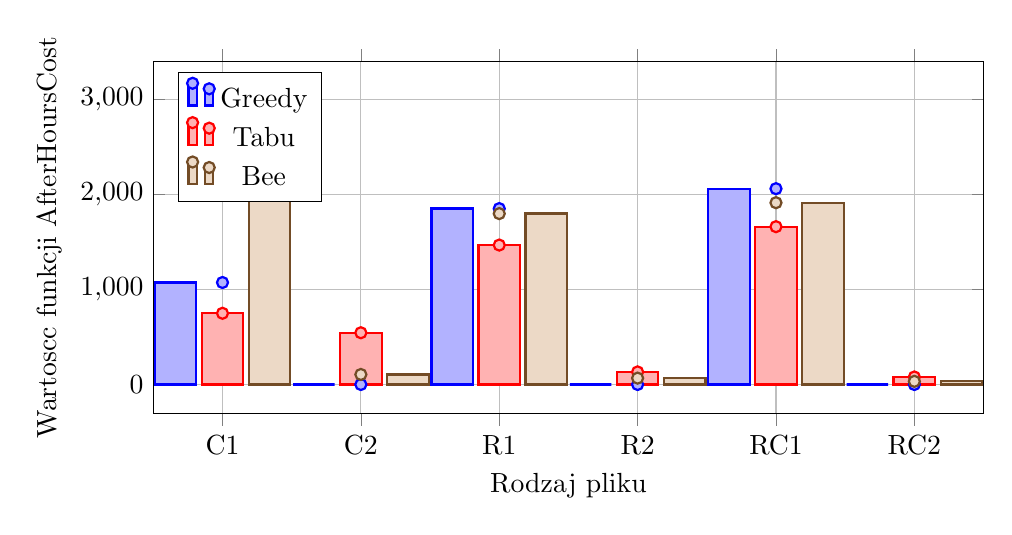
\begin{tikzpicture}
\begin{axis}[
xlabel = {Rodzaj pliku},
ylabel = {Wartoscc funkcji AfterHoursCost},
legend pos = north west,
grid = both,
width=1\linewidth,
height=0.5\linewidth,
ybar,
bar width=15pt,
symbolic x coords={C1,C2,R1,R2,RC1,RC2,},
xtick=data
]
\addplot + [mark = *, thick] coordinates
    {
(C1,1073.3333333333333)(C2,0.0)(R1,1850.8333333333333)(R2,0.0)(RC1,2060.375)(RC2,0.0)};
\addlegendentry
{Greedy}
\addplot + [mark = *, thick] coordinates
    {
(C1,749.5555555555555)(C2,544.625)(R1,1467.25)(R2,132.54545454545453)(RC1,1660.625)(RC2,79.375)};
\addlegendentry
{Tabu}
\addplot + [mark = *, thick] coordinates
    {
(C1,3093.6666666666665)(C2,105.75)(R1,1798.1818181818182)(R2,67.27272727272727)(RC1,1912.875)(RC2,33.5)};
\addlegendentry
{Bee}
\end{axis}
\end{tikzpicture}
\caption
{Porownanie srednich wartosci AfterHoursCost algorytmow dla kazdego rodzaju pliku}
\label{fig:mean_AfterHoursCost_comparision}
\end{figure}
